\documentclass{article}
\usepackage[utf8]{inputenc}
\usepackage{graphicx}
\usepackage{float}
\usepackage{amsmath}
\usepackage{amssymb}
\usepackage{listings}
\usepackage{color}
\usepackage{siunitx}
\usepackage{comment}
\usepackage{hyperref}
\usepackage{enumitem}
\usepackage{cite}
\usepackage{environ}
\usepackage{caption}
\usepackage{subcaption}
\newcommand\tab[1][1cm]{\hspace*{#1}}

\makeatletter
\NewEnviron{widerequation}{%
  \begin{equation*}
  \sbox\z@{\let\label\@gobble$\displaystyle\BODY$}
  \makebox[\textwidth]{%
    \begin{minipage}{\dimexpr\wd\z@+3em}
    \vspace{-\baselineskip}
    \begin{equation*}
    \BODY
    \end{equation*}
    \end{minipage}%
  }
  \end{equation*}
}
\makeatother

\definecolor{codegreen}{rgb}{0,0.6,0}
\definecolor{codegray}{rgb}{0.5,0.5,0.5}
\definecolor{codepurple}{rgb}{0.58,0,0.82}
\definecolor{backcolour}{rgb}{0.95,0.95,0.92}
 
\lstdefinestyle{mystyle}{
    backgroundcolor=\color{backcolour},   
    commentstyle=\color{codegreen},
    keywordstyle=\color{magenta},
    numberstyle=\tiny\color{codegray},
    stringstyle=\color{codepurple},
    basicstyle=\footnotesize,
    breakatwhitespace=false,         
    breaklines=true,                 
    captionpos=b,                    
    keepspaces=true,                 
    numbers=left,                    
    numbersep=5pt,                  
    showspaces=false,                
    showstringspaces=false,
    showtabs=false,                  
    tabsize=2
}

\lstset{style=mystyle}

\title{TTK22 Software Toolchain for Networked Vehicle Systems Project}
\author{Henning Ødeby Karlsen}
\date{November 2020}

\begin{document}

\maketitle

%
% GRAPHICS
%

% \begin{figure}[H]
%     \centering
%     \includegraphics[width=8cm]{MATLAB/bike.png}
%     \caption{The bike model, from the assignment paper}
%     \label{fig:pendulum_on_cart}
% \end{figure}

%
% MATRIX ADDITION ETC
%
% $$ M
% \begin{bmatrix}
%     \ddot\phi\\
%     \ddot\delta
% \end{bmatrix}
% +Cv_0
% \begin{bmatrix}
%     \dot\phi\\
%     \dot\delta
% \end{bmatrix}
% +(K_0+K_2v^2_0)
% \begin{bmatrix}
%     \phi\\
%     \delta
% \end{bmatrix}
% =
% \begin{bmatrix}
%     0\\
%     T
% \end{bmatrix}
% $$

%
% EQUATIONS
%

% $$ \ddot\phi = -\frac{\dot\phi Cv_0 }{M} - \frac{(K_0+K_2v^2_0)\phi}{M}$$
% $$ \ddot\delta = \frac{T}{M} -\frac{\dot\delta Cv_0 }{M} - \frac{(K_0+K_2v^2_0)\delta}{M}$$

%$$ 
% A =
% \begin{bmatrix}
%     0 && 0 && 1 && 0\\
%     0 && 0 && 0 && 1\\
%     - \frac{(K_0+K_2v^2_0)}{M} && 0 && -\frac{Cv_0 }{M} && 0\\
%     0 && - \frac{(K_0+K_2v^2_0)}{M} && 0 && -\frac{Cv_0 }{M} 
% \end{bmatrix}
% $$
%$$ 
% A =
% \begin{bmatrix}
%     0 && 0 && 1 && 0\\
%     0 && 0 && 0 && 1\\
%     - \frac{(K_0+K_2v^2_0)}{M} && 0 && -\frac{Cv_0 }{M} && 0\\
%     0 && - \frac{(K_0+K_2v^2_0)}{M} && 0 && -\frac{Cv_0 }{M} 
% \end{bmatrix}
% $$

%
% 3x3 MATRIX
%

% $$ 
% A =
% \begin{bmatrix}
%     0 && 0 && 1 && 0\\
%     0 && 0 && 0 && 1\\
%     - \frac{(K_0+K_2v^2_0)}{M} && 0 && -\frac{Cv_0 }{M} && 0\\
%     0 && - \frac{(K_0+K_2v^2_0)}{M} && 0 && -\frac{Cv_0 }{M} 
% \end{bmatrix}
% $$

%
% CODE 
%

% \lstinputlisting[language=matlab]{MATLAB/output.m}
% \lstinputlisting[language=matlab, firstline=94, lastline=113]{MATLAB/bike.m}

%
% TABLES
%

% https://no.overleaf.com/learn/latex/Tables

% \begin{center}
%     \begin{tabular}{ |c|c|c| } 
%      \hline
%      cell1 & cell2 & cell3 \\ 
%      cell4 & cell5 & cell6 \\ 
%      cell7 & cell8 & cell9 \\ 
%      \hline
%     \end{tabular}
%\end{center}

%
% TEXT FORMATTING
%

% https://www.overleaf.com/learn/latex/bold,_italics_and_underlining

%
% LISTS WITH a,b,c etc.
%

% \begin{enumerate}[label=(\alph*)]
%     \item What is the size of the training set used?\\
%     \textit{\textbf{Answer:} 300}
%     \item Which class had the highest number of errors?\\
%     \textit{\textbf{Answer:} Class 9 out of 10 classes, with 10 errors, assuming an error is anything that lies outside of the diagonal, where correct class = predicted class}
%     \item What was the overall percentage correct?\\
%     \textit{\textbf{Answer:} Overall correct percentage was 86.667\% }    
% \end{enumerate}

%
% CASES (Squig over flere linjer)
%

% \begin{cases}
%     \pi^{d/2}/(d/2)!, &  d \text{ even}\\
%     2^d\pi^{(d-1)/2}\frac{d-1}{2}!/d!, &  d \text{ odd}\\
% \end{cases} 

%
% Fotnote
%

% \footnote{Denne teksten blir stående nede, også kommer det et tall der dette står.}
% Har litt andre funksjoner også https://www.overleaf.com/learn/latex/footnotes

%
% Hyperlenker https://www.overleaf.com/learn/latex/hyperlinks
%

% \href{URL}{tekst}



\newpage
\section{Approach}
For this project, I wanted to see what would be required for SINTEFs JavaScript Graphical User Interface, Aqueous, to communicate with DUNE, instead of the FhSim it is set up to communicate.
\subsection{Aqueous}
Aqueous is developed in the JavaScript framework React, and is used as the interface between the control system of one of SINTEFs ROVs.
The GUI has two components. The first is a Video HUD for displaying the video feed from the ROV as well as visualize the location of the ROV. 
The second is a control view for visualizing the current control situation, as well as issuing some controls. 
In the control view, the user can switch between three different modes: NF (NetFollowing), DP (DynamicPositioning) and Manual.
The manual control and changing of biases in the other modes are done either by a gamepad or the keyboard. 

\begin{figure}[H]
    \centering
    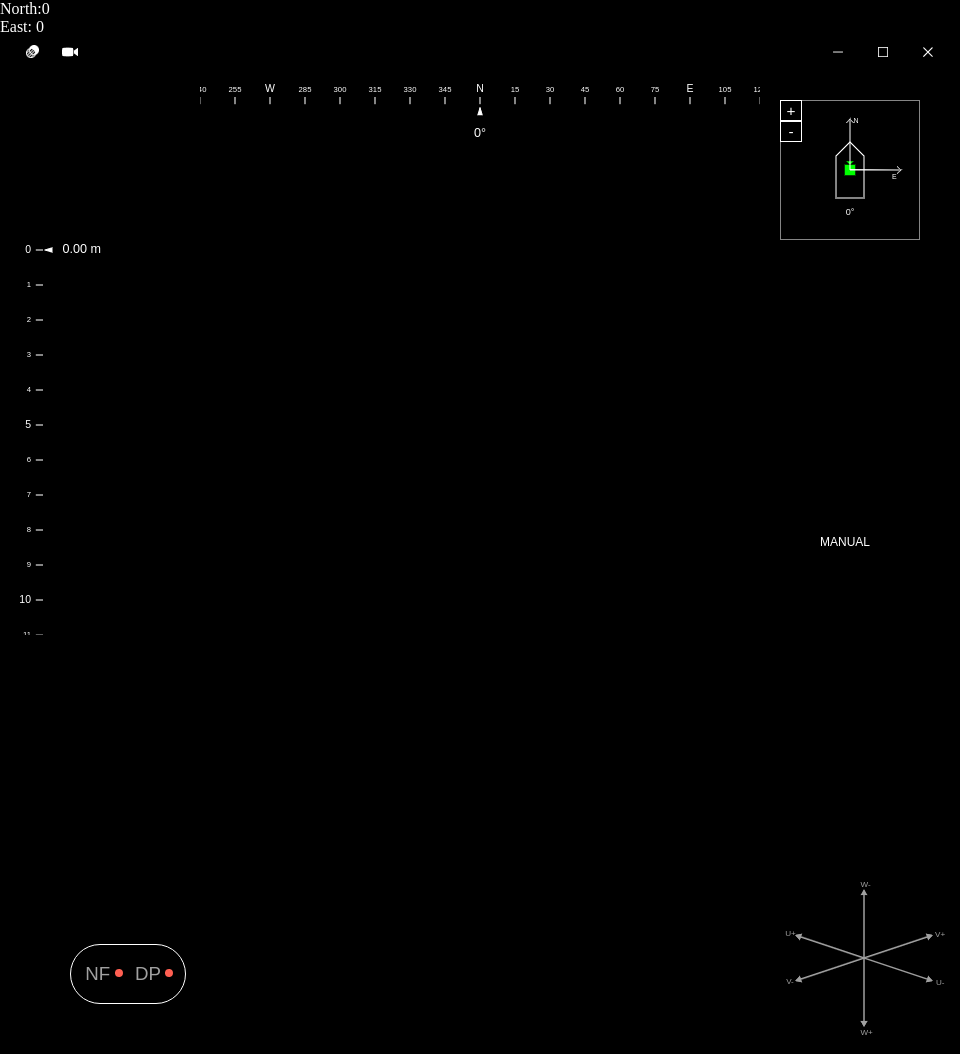
\includegraphics[width=0.75\textwidth]{AqHUD.png}
    \caption{The video HUD. When no ROV/video is connected, the screen is black}
    \label{fig:HUD}
\end{figure}

\begin{figure}[H]
    \centering
    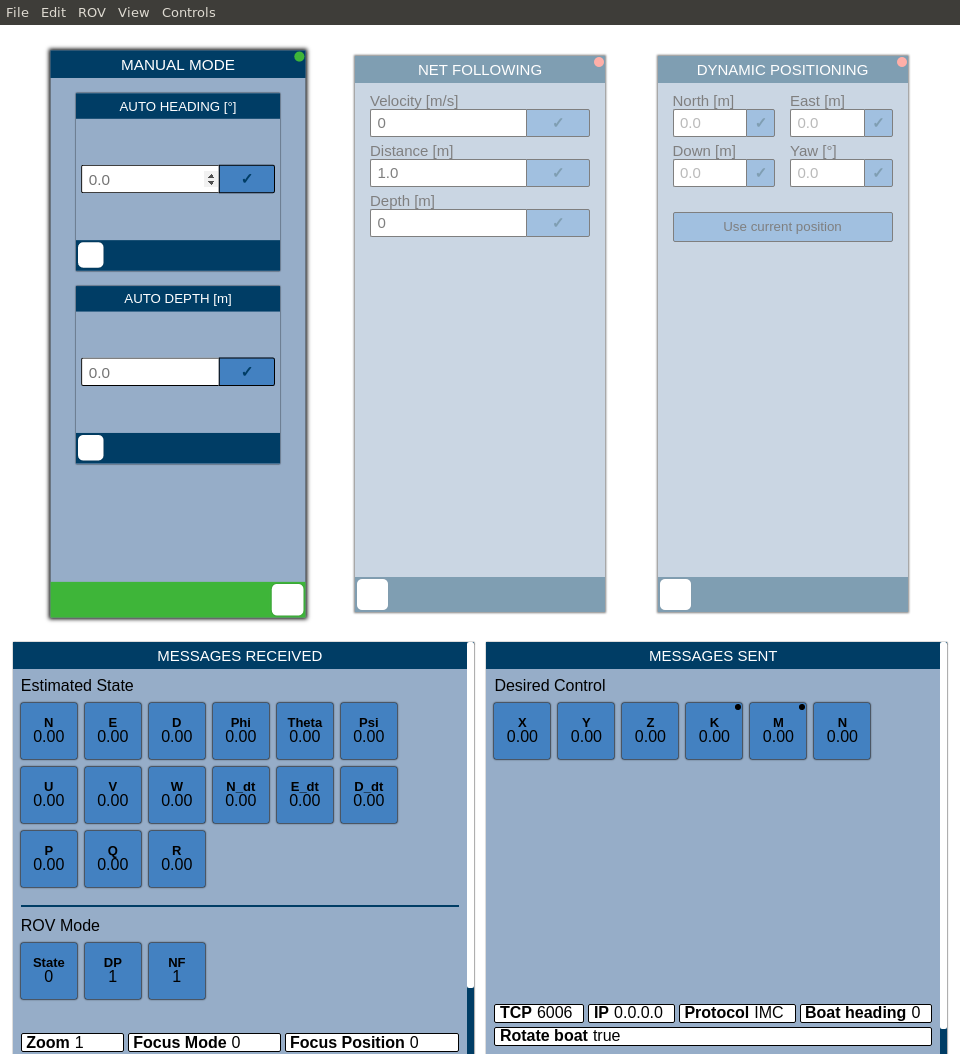
\includegraphics[width=\textwidth]{AqControl.png}
    \caption{The control view when no ROV is connected.}
    \label{fig:control}
\end{figure}
\noindent
The relevant parts of Aqueous for this project is the communication with FhSim, which I will look into changing in this project, such that it can be used to communicate with DUNE.
\subsubsection{Communcations}
Aqueous is already set up to use IMC for communication with FhSim, but it uses a few custom messages, and does not follow the same "structure" "Paradigme?" "Taxionomy" of communication as DUNE.
I was told by people at SINTEF that Aqueous would not work "out of the box" with DUNE. 
So I started with trying to get them connected through TCP. 
After finding the right addresses I was able to get a connection between them, but Aqueous instantly crashed as it was not prepared to receive unknown messages.
I started by looking into the way Aqueous receives these messages, such that I could add support for the 


\section{Organization}

\section{Results}


% \bibliography{references.bib}{}
% \bibliographystyle{abbrv}
\end{document}